\section{Results}
\subsection{Result from tracking}

How well it tracked objects and how many it could track at the same time.

\subsection{Analysing training different configurations and their charts}

Different model configuration and the test results. Charts of accuracy and loss.

\subsection{Results from doing object detection in matlab}
A Matlab script was tried in order to find possible ways of segmenting out regions containing objects in an image. The output segments would then each be classified separately. This way we would have both object locations and classifications on each object. \ref{fig:matlabImages} shows an example of this. However, results from this were highly unpredictable and the parameters were too dependent on lighting, shadows, the background among other features. Hence, this method was scrapped.

\subsection{Results from doing object detection with Turi}
Because of the vast amount of possible use cases it was decided to scale the objective down. The model was trained only on a few floor backgrounds. 

The mean average precision from the different models that were trained were observed and can be read in table \ref{table:mAP}. 

\begin{table}[h]
\centering
\begin{tabular}{ |c|c| } 
 \hline
 Percentage of training images used & mean\_average\_precision  \\ 
 \hline
 5\% & 0.17064 \\ 
 \hline
 20\% & 0.39269 \\ 
 \hline
 40\% & 0.40595 \\
 \hline
 50\% & 0.47397
 \hline
\end{tabular}
\caption{Mean average precision depending on the amount of training data used. 100\% corresponds to 926 images.}
\label{table:mAP}
\end{table}

These values can then be plotted giving us the graph shown in figure

[SAMPLE BILD TILLS VI HAR GENERERAT KORREKT PLOT]
\begin{figure}[hbtp]
\begin{center}
\includegraphics[width = 0.32\textwidth]{./Images/3dscanning1.png}
\caption{Mean Average Precision plotted against the amount of training data used. 100\% corresponds to 926 images.}
\label{fig:mAP}
\end{center}
\end{figure}

[iNCLUDE IMAGES FROM TESTING  IN TURI]

\subsection{Rendered nodes in ARScene and how stable they were}
Precision when doing the hit tests

How well the nodes stayed in their place (depending on environment?)

\subsection{Overall performance of the app}

What is the peek performance?

\subsection{User tests}

A user survey was done in order to evaluate the performance of the application. By having a multitude of interested people booking time slots for a ten minute testing period, a decent amount of sample data could be gathered and evaluated. Figures \ref{fig:question1} to \ref{fig:question6} show bar charts and pie charts representing the answers gathered from the participants to some of the questions they were asked. 

\begin{figure}[hbtp]
\begin{center}
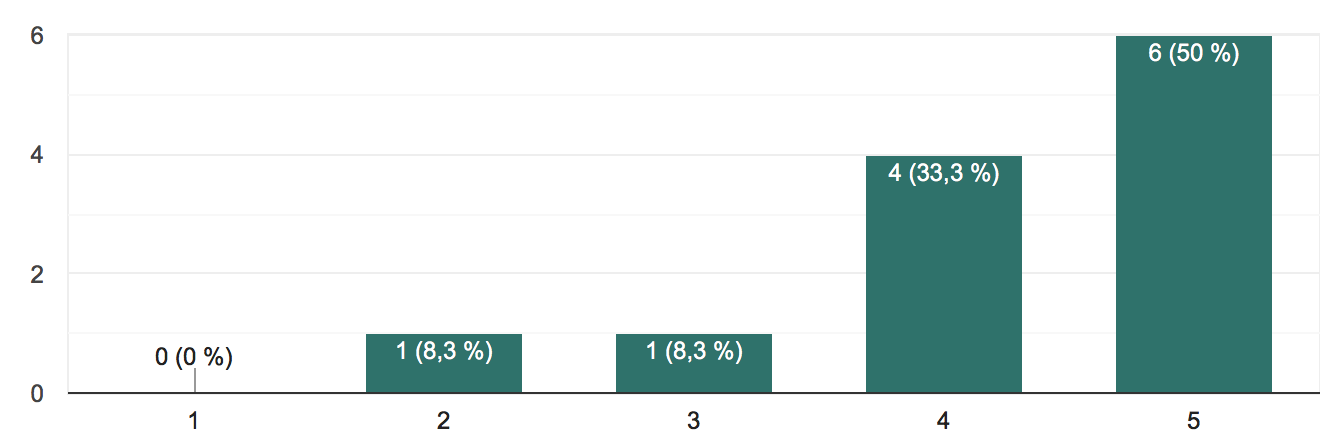
\includegraphics[width = 0.9\textwidth]{./Images/easyToGetToNext.png}
\caption{Results from when users were asked "How easy was it to understand how to get to the next step?"}
\label{fig:question1}
\end{center}
\end{figure}

\begin{figure}[hbtp]
\begin{center}
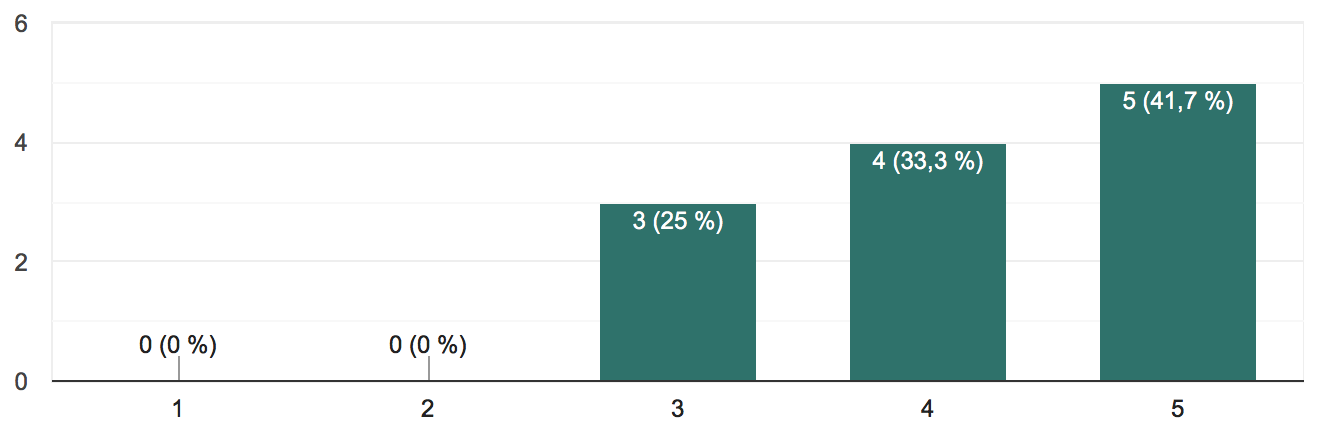
\includegraphics[width = 0.9\textwidth]{./Images/easyToUnderstand.png}
\caption{Results from when users were asked "How easy was it to understand how the pieces fit together?"}
\label{fig:question2}
\end{center}
\end{figure}

\begin{figure}[hbtp]
\begin{center}
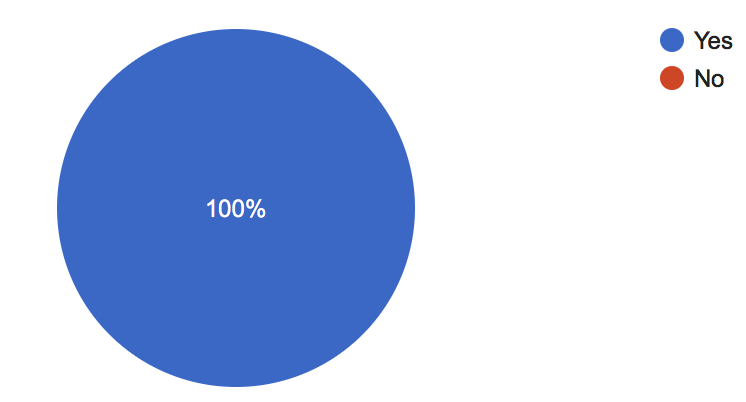
\includegraphics[width = 0.6\textwidth]{./Images/knowToSkip.png}
\caption{Results from when users were asked "Did you know that you could skip instructions?"}
\label{fig:question3}
\end{center}
\end{figure}

\begin{figure}[hbtp]
\begin{center}
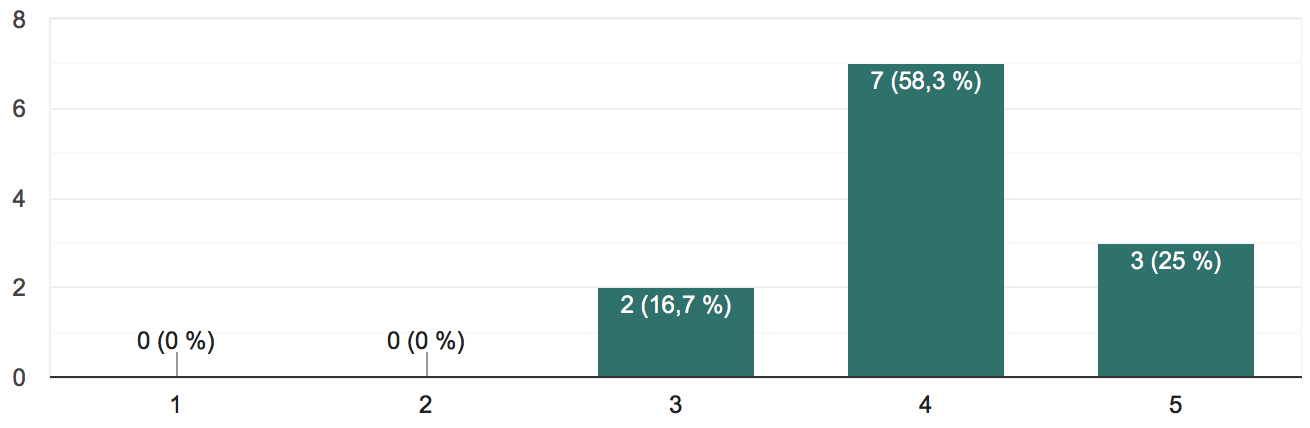
\includegraphics[width = 0.9\textwidth]{./Images/easyToUse.png}
\caption{Results from when users were asked "How easy was it to understand how to get to the next step?"}
\label{fig:question4}
\end{center}
\end{figure}

\begin{figure}[hbtp]
\begin{center}
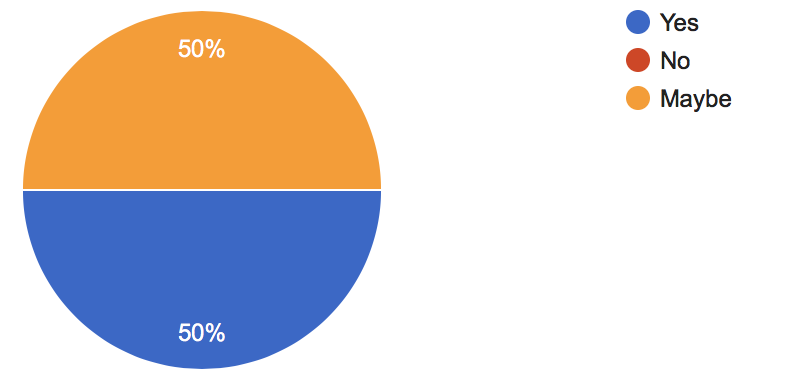
\includegraphics[width = 0.6\textwidth]{./Images/comparedTo.png}
\caption{Results from when users were asked "Compared to using paper instructions, did the app make it easier to understand how to put together the furniture?"}
\label{fig:question5}
\end{center}
\end{figure}

\begin{figure}[hbtp]
\begin{center}
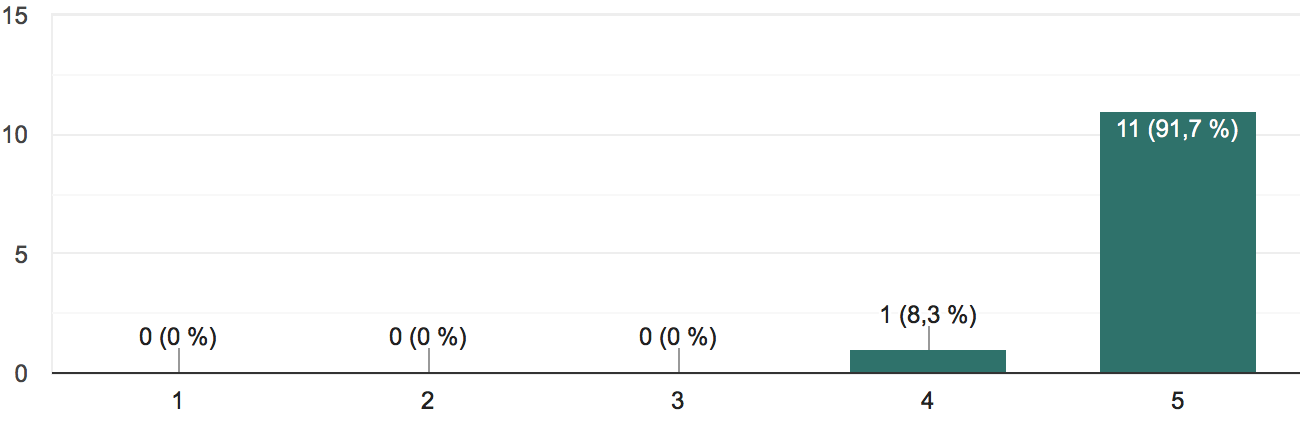
\includegraphics[width = 0.9\textwidth]{./Images/potential.png}
\caption{Results from when users were asked "What potential do you see in this app?"}
\label{fig:question6}
\end{center}
\end{figure}

What people liked and found interesting


what people disliked and found confusing


Suggestions for improvements



Sammanställ info: \\

How to make instructions easy to understand in AR

Green rectangles were confusing

Back button?

People trying to rotate the object

The app needs glasses to make it hands free

Voice instructions

Confusing when the part was in unsupported orientation








\newpage